\documentclass[a4j,12]{jarticle}
\usepackage{exp1}

%\pagestyle{empty}
%%%%%%%%%%%%%%%%%%%%%
%%%レポート作成者情報の入力
%%%班
\def\group{グループ番号}
%%%学籍番号
\def\idnumber{1315193T}
%%%氏名
\def\name{薛 宇航}
%%%実験月日月
\def\expmontho{月}
\def\expdayo{日}
%%%実験月日
\def\expmontht{月}
\def\expdayt{日}
%%%実験月日
\def\expmonthth{月}
\def\expdayth{日}
%%%レポート提出月日
\def\deadlinem{12}
\def\deadlined{21}
%%%共同実験者1
\def\groupmembero{1305194T 中山 峻一}
%%%共同実験者2 居なかった場合には{}だけにする.
\def\groupmembert{1385195T 藤原 巧}
%%%共同実験者3 居た場合には{}内に学籍番号と氏名を入力する.
\def\groupmemberh{1365196T 和田 佳大}
%%%%%%%%%%%%%%%%%%%


\begin{document}

\title{
  \vspace{1cm}{\LARGE 平成27年度}\\
  % \vspace{1em}
  \begin{spacing}{1.5}
    {\Huge ディジタル信号処理課題4}\\
    {\huge --適応フィルタ--}
  \end{spacing}
  \author{}
  \date{}
}%%表紙の情報、、入力忘れないように
\maketitle
\vspace{5cm}
       {\Large
         \begin{spacing}{1.2}
           \hspace{20em}\underline{レポート提出日:\deadlinem 月\deadlined 日}\\
           \hspace{20em}\underline{学籍番号:\idnumber}\\
           \hspace{20em}\underline{氏  名:\name}\\
         \end{spacing}
       }
       

       \thispagestyle{empty}
       \newpage
       \setcounter{page}{1}      %ページ番号リセット
       
       


       \section{原理}
       \subsection{音響システム}
       空気中の音の伝搬は、大気圧の変化が縦波として伝搬するものであり、この伝搬を線形であるとみなす。またスピーカーからマイクロホンまでん2点間の音の伝達特性は、物体の移動や気温変化などに伴い変化する量であるので、厳密には線形時変システムと考えられる。しかし、短い時間範囲であれば、その変化は十分小さいと考え、時不変システムとしてみなす。このとき、スピーカーからの信号をx[n]、スピーカーとマイクロホンの2点間の音の伝達特性をh[k]とすると、マイクロホンにて観測される信号d[n]は、二つの信号x[n]とh[k]の畳み込みによって、以下の式(1)ように得られる。

       \begin{equation}
         d[n] \approx \sum_k h[k]x[n-k]
       \end{equation}
       ここで上式では、人の声は存在せず、マイクロホンにはスピーカーの音のみ観測されるとしている。もし人の声も存在する場合は、マイクロホンにて観測される信号d[n]は、スピーカー音と、音声の加算によって表現される。これは下の式(2)のように示す。
       \begin{equation}
         d[n] \approx \sum_k h[k]x[n-k]+s'[n]         
       \end{equation}
       ここで、 $s'[n]$は、音声s[n]に伝達特性を畳み込んだ信号とする、式(2)のフィルタ係数h[k]がわかれば、人の声に重畳したスピーカーからの音楽などの「音」を消して、人の声だけを聞くことができる。実際には手間のかかる作業隣る。そこで、ここではLMS(Least Mean Square)アルゴリズムを用いてフィルタ係数h[K]を求める。
       \subsection{正規化LMSアルゴリズムによる音楽消去}
       LMSアルゴリズムでは、逐次的にフィルタ係数を求める。時刻nでのフィルタ係数を$h_n[k]$とすると、式(1)の左辺と右辺の誤差は
       \begin{equation}
         e[n]=d[n]-\sum_{k=0}^{K-1}h_n[k]x[n-k]
       \end{equation}
       フィルタ係数の更新する式は以下のようになる。
       \begin{equation}
         h_{n+1}[k]=h_n[k]+ \frac{\alpha}{||x[n]||^2}×e[n]×x[n-k]
       \end{equation}


       \section{課題1}
       \subsection{課題内容}
              web pageにサンプルデータを置いてある。サンプルデータを使い(学番の下一桁が奇数のため、サンプル1となる)、サンプルデータの最初の20秒間、NLMSを用いてフィルタ係数を推定せよ。適応フィルタの初期値は0、$\alpha$=0.02とせよ \par
       適応フィルタの次数Kを10,20,・・・50,・・・とした場合、誤差値がどのように変わっているかを述べよ。
       \subsection{解答内容}
       適正フィルタの次数Kが大きくなるにつれて、誤差eの振動が小さくなってくる。それぞれ次数Kを10、20、50にした時、誤差eはそれぞれ以下の図1に示すようになる。
       \begin{figure}[htpb]
         \begin{center}
           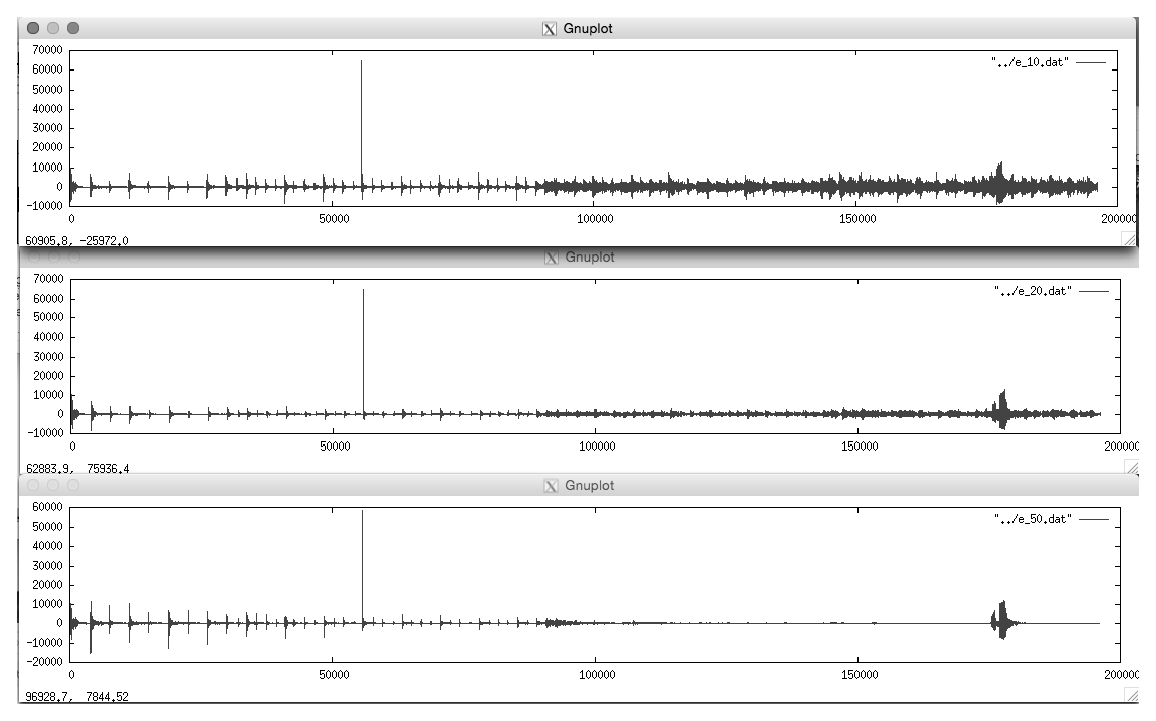
\includegraphics[width=15cm]{e.eps}%%widethで大きさ変わる、
           \caption{次数の変化によって誤差値の変わり方}
           \label{micon}
         \end{center}
       \end{figure}
       
       なお、今の課題で使用するプログラムは以下のようになる。
       \begin{lstlisting}[caption=課題1で使用するプログラム,label=rp1]
#include <stdio.h>
#include <stdlib.h>
#include <math.h>


#define Pi 3.14159265358979
#define alpha 0.01
#define K 50   //changed everytime to ensure the output
#define MAX 300000

int main(){
  char d_filename[128]="observed_song1.raw";//short
  char x_filename[128]="song1.raw";//short
  char e_filename[128]="e.raw";
  
  int k,n,size_d,size_x;
  
  short *d,*x,s[MAX],tmp;
  FILE *file_input;
  FILE *file_output;

  double e[160000];
  double h_n[K]={0},h_n1[K]={0},norm;
  //double h;


  //operation of d
  if((file_input=fopen(d_filename,"rb"))==NULL){
    fprintf(stderr,"Cannot read %s .\n",d_filename);exit(-1);
  }
  size_d=fread(s,sizeof(short),MAX,file_input);
  d=(short *)calloc(size_d,sizeof(float));
  fclose(file_input);
  if((file_input=fopen(d_filename,"rb"))==NULL){
    fprintf(stderr,"Cannot read %s .\n",d_filename);exit(-1);
  }
  fread(d,sizeof(short),size_d,file_input);
  fclose(file_input);





  //operation of x
  if((file_input=fopen(x_filename,"rb"))==NULL){
    fprintf(stderr,"Cannot read %s.\n",x_filename);exit(-1);
  }
  size_x=fread(s,sizeof(short),MAX,file_input);
  x=(short *)calloc(size_x,sizeof(short));
  fclose(file_input);
  if((file_input=fopen(x_filename,"rb"))==NULL){
    fprintf(stderr,"Cannot read %s.\n",x_filename);exit(-1);
  }
  fread(x,sizeof(short),size_x,file_input);
  fclose(file_input);
  

  for(n=0;n<size_d;n++){
  
    

    
    e[n]=(double)d[n];
    //∵at this time,n=n+1 ∴update the h_n1 to h_n
    for(k=0;k<K;k++){
      h_n[k]=h_n1[k];
      e[n]-=h_n[k]*x[n-k];

    }
    norm=0.0;//initial norm
    for(k=0;k<K;k++){
      if(n>k){
	norm+=x[n-k]*x[n-k];
      }
    }
    
    for(k=0;k<K;k++){
      h_n1[k]=h_n[k];
      if(norm==0){
	  norm = 1;
      }
      h_n1[k]=h_n[k]+alpha*e[n]*x[n-k]/norm;
    }
  }
  
  
  
  if((file_output = fopen(e_filename,"wb")) == NULL){
    fprintf(stderr, "Cannot write %s\n", e_filename);  exit(-1);
  }
  for(n=0;n<size_d;n++){
    //printf("%lf\n",e[n]);  //use gnuplot to plot error
    tmp = (short)e[n];
    fwrite(&tmp, sizeof(short), 1, file_output);
  }
  
  fclose(file_output);





  

  free(d);
  free(x);
  return 0;
}

         
       \end{lstlisting}
       \section{課題2}
       \subsection{課題内容}
       2秒、10秒、20秒の時に推定されたフィルタ係数、及び正解のh[k]を表示して、時刻とともに正解のh[k]に近づいていることを確認せよ。
       \subsection{解答内容}
       K=50の時、2秒、10秒、20秒の時に推定されたフィルタ係数及び正解のh[k]を同じ図表にプロットして、以下の図2のようになります。
       \begin{figure}[htpb]
         \begin{center}
           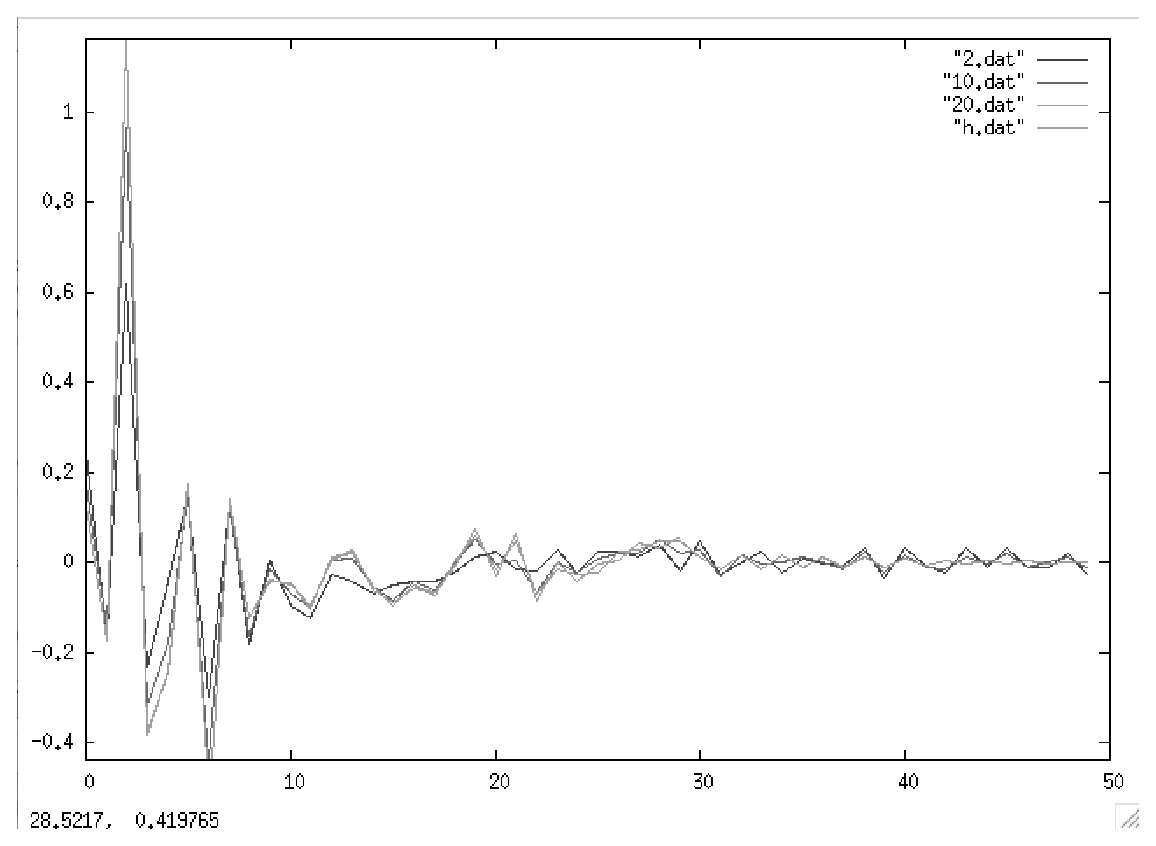
\includegraphics[width=15cm]{h.eps}%%widethで大きさ変わる、
           \caption{K=50の推定フィルタ係数と正解の比較}
           \label{micon}
         \end{center}
       \end{figure}
       本レポートはtexによって作成されたため、引用する画像を全てepsファイルの白黒になります。図からわかりにくいと思いますが、時間とともに正解のh[k]に近づくことが確かである。なお、本レポートと共に、カラー画像も一緒に添付し、指定メールアドレスに送る。
       
       \begin{lstlisting}[caption=課題2で使用するプログラム,label=rp2]
#include <stdio.h>
#include <stdlib.h>
#include <math.h>


#define Pi 3.14159265358979
#define alpha 0.01
#define K 50   //changed everytime to ensure the output
#define MAX 300000

int main(){
  char d_filename[128]="observed_song1.raw";//short
  char x_filename[128]="song1.raw";//short
  char h_filename[128]="imp.dat";//float
  char e_filename[128]="e.raw";
  
  
  int k,n,size_h,size_d,size_x;
  
  short *d,*x,s[MAX],tmp;
  float *h,f[MAX];
  FILE *file_input;
  FILE *file_output;
  
  double e[160000];
  double h_n[K]={0},h_n1[K]={0},norm;
  //double h;

  
  //operation of d
  if((file_input=fopen(d_filename,"rb"))==NULL){
    fprintf(stderr,"Cannot read %s .\n",d_filename);exit(-1);
  }
  size_d=fread(s,sizeof(short),MAX,file_input);
  d=(short *)calloc(size_d,sizeof(float));
  fclose(file_input);
  if((file_input=fopen(d_filename,"rb"))==NULL){
    fprintf(stderr,"Cannot read %s .\n",d_filename);exit(-1);
  }
  fread(d,sizeof(short),size_d,file_input);
  fclose(file_input);





  //operation of x
  if((file_input=fopen(x_filename,"rb"))==NULL){
    fprintf(stderr,"Cannot read %s.\n",x_filename);exit(-1);
  }
  size_x=fread(s,sizeof(short),MAX,file_input);
  x=(short *)calloc(size_x,sizeof(short));
  fclose(file_input);
  if((file_input=fopen(x_filename,"rb"))==NULL){
    fprintf(stderr,"Cannot read %s.\n",x_filename);exit(-1);
  }
  fread(x,sizeof(short),size_x,file_input);
  fclose(file_input);



  
    //operation of h
  if((file_input=fopen(h_filename,"rb"))==NULL){
    fprintf(stderr,"Cannot read %s.\n",h_filename);exit(-1);
  }
  size_h=fread(f,sizeof(float),MAX,file_input);
  h=(float *)calloc(size_h,sizeof(float));
  fclose(file_input);
  if((file_input=fopen(h_filename,"rb"))==NULL){
    fprintf(stderr,"Cannot read %s.\n",h_filename);exit(-1);
  }
  fread(h,sizeof(float),size_h,file_input);
  fclose(file_input);


  
  //for(k=0;k<size_h;k++){
  // printf("%lf\n",h[k]);
  //}
  
  
  for(n=0;n<size_d;n++){
    if(n==8000*10){
     for(k=0;k<K;k++){
    	printf("%lf\n",h_n[k]);}
    }


    
    e[n]=(double)d[n];
    //∵at this time,n=n+1 ∴update the h_n1 to h_n
    for(k=0;k<K;k++){
      h_n[k]=h_n1[k];
      e[n]-=h_n[k]*x[n-k];

    }
    norm=0.0;//initial norm
    for(k=0;k<K;k++){
      if(n>k){
	norm+=x[n-k]*x[n-k];
      }
    }
    
    for(k=0;k<K;k++){
      h_n1[k]=h_n[k];
      if(norm==0){
	  norm = 1;
      }
      h_n1[k]=h_n[k]+alpha*e[n]*x[n-k]/norm;
    }
  }
  
  
  
  if((file_output = fopen(e_filename,"wb")) == NULL){
    fprintf(stderr, "Cannot write %s\n", e_filename);  exit(-1);
  }
  for(n=0;n<size_d;n++){
    //printf("%lf\n",e[n]);  //use gnuplot to plot error
    tmp = (short)e[n];
    fwrite(&tmp, sizeof(short), 1, file_output);
  }
  

  fclose(file_output);





  

  free(d);
  free(x);
  free(h);
  return 0;
}

       \end{lstlisting}
       \section{課題3}
       \subsection{課題内容}
       21秒から23秒の間に人が発話を行っている。この時間区間に置けるマイクロホンの観測信号d[n]、スピーカーからの音楽を除去した信号$s'[n]$、クリーン音声信号s[n]、これら3つの信号の波形及びスペクトプログラムを表示せよ。
       \subsection{解答内容}
       web pageに置かれてる音声信号ファイルを読み込み、21秒から23秒の間だけ操作して、d[n]、s[n]、及びs'[n]の波形及びスペクトログラムをそれぞれ図3、図4、図5に示す。
       \begin{figure}[htpb]
         \begin{center}
           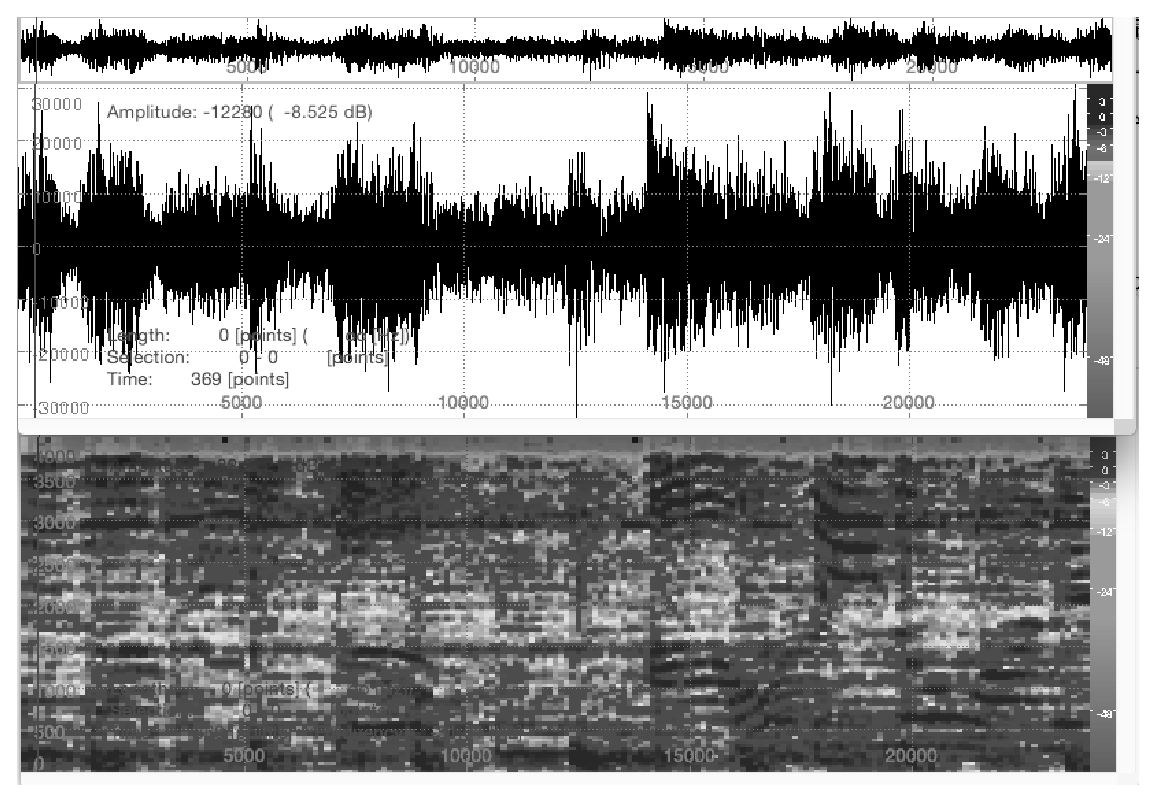
\includegraphics[width=15cm]{d.eps}%%widethで大きさ変わる、
           \caption{d[n]の波形及びスペクトル(20s~23s)}
           \label{micon}
         \end{center}
       \end{figure}
       \begin{figure}[htpb]
         \begin{center}
           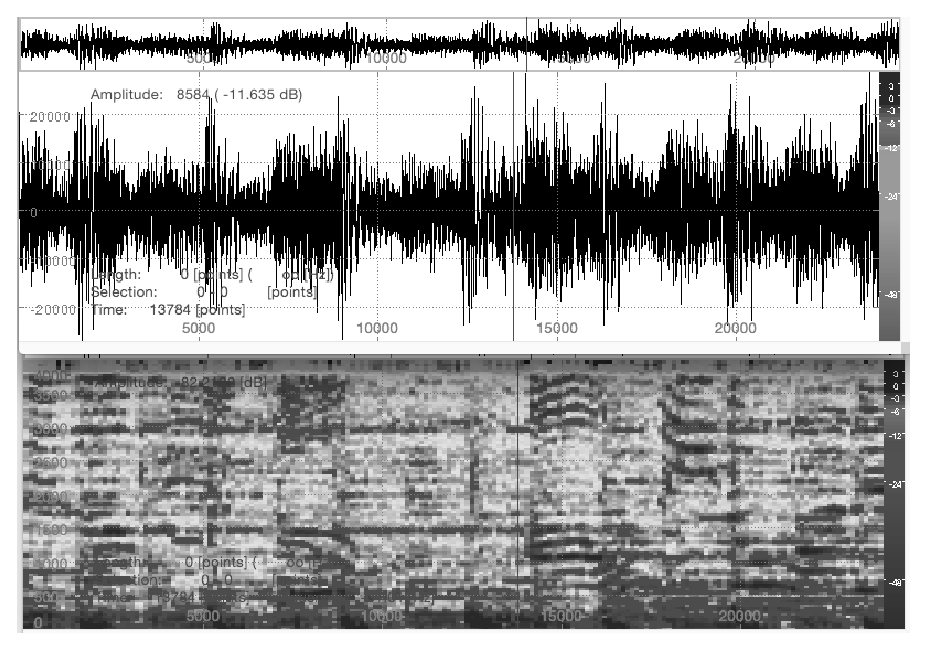
\includegraphics[width=15cm]{s.eps}%%widethで大きさ変わる、
           \caption{s[n]の波形及びスペクトル(20s~23s)}
           \label{micon}
         \end{center}
       \end{figure}
       \begin{figure}[htpb]
         \begin{center}
           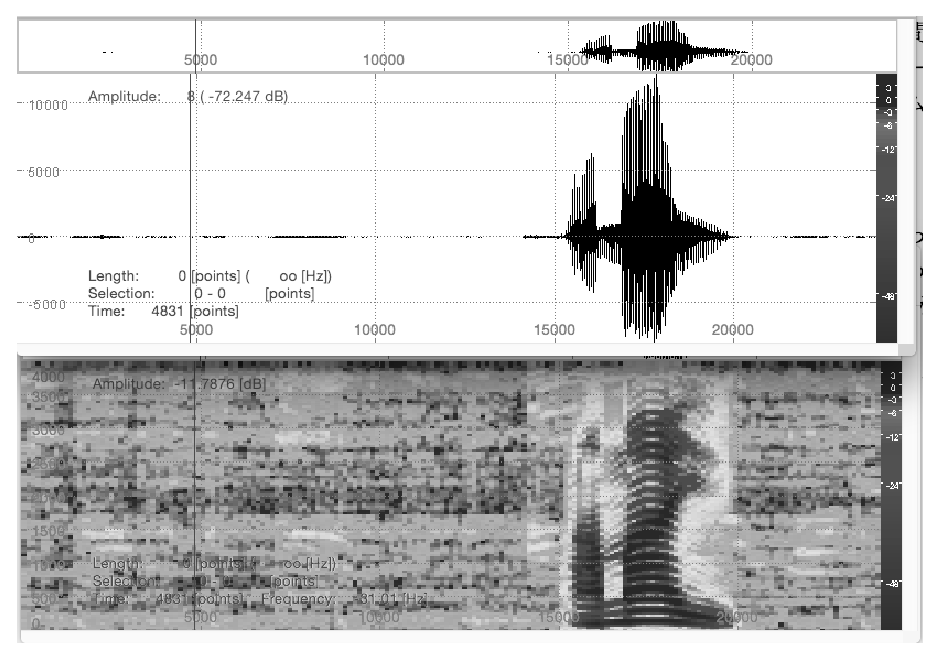
\includegraphics[width=15cm]{s_s.eps}%%widethで大きさ変わる、
           \caption{s'[n]の波形及びスペクトル(20s~23s)}
           \label{micon}
         \end{center}
       \end{figure}

       

       \par
       なお、本課題に使用するプログラムは以下のようになります。
       \begin{lstlisting}[caption=課題3で使用するプログラム,label=rp3]
#include <stdio.h>
#include <stdlib.h>
#include <math.h>


#define Pi 3.14159265358979
#define alpha 0.01
#define K 50   //changed everytime to ensure the output
#define MAX 300000

int main(){
  char d_filename[128]="observed_song1.raw";//short
  char x_filename[128]="song1.raw";//short
  char e_filename[128]="e.raw";
  char d_3[128]="d.raw";
  char s_3[128]="s.raw";
  char s_s_3[128]="s_s.raw";
  
  int k,n,size_d,size_x;
  
  short *d,*x,s[MAX],tmp;
  FILE *file_input;
  FILE *file_outputd;
  FILE *file_outputs;
  FILE *file_outputs_s;

  double e[160000];
  double h_n[K]={0},h_n1[K]={0},norm;
  //double h;



  //operation of d
  if((file_input=fopen(d_filename,"rb"))==NULL){
    fprintf(stderr,"Cannot read %s .\n",d_filename);exit(-1);
  }
  size_d=fread(s,sizeof(short),MAX,file_input);
  d=(short *)calloc(size_d,sizeof(float));
  fclose(file_input);
  if((file_input=fopen(d_filename,"rb"))==NULL){
    fprintf(stderr,"Cannot read %s .\n",d_filename);exit(-1);
  }
  fread(d,sizeof(short),size_d,file_input);
  fclose(file_input);





  //operation of x
  if((file_input=fopen(x_filename,"rb"))==NULL){
    fprintf(stderr,"Cannot read %s.\n",x_filename);exit(-1);
  }
  size_x=fread(s,sizeof(short),MAX,file_input);
  x=(short *)calloc(size_x,sizeof(short));
  fclose(file_input);
  if((file_input=fopen(x_filename,"rb"))==NULL){
    fprintf(stderr,"Cannot read %s.\n",x_filename);exit(-1);
  }
  fread(x,sizeof(short),size_x,file_input);
  fclose(file_input);
  
  
  for(n=0;n<size_d;n++){

    e[n]=(double)d[n];
    //∵at this time,n=n+1 ∴update the h_n1 to h_n
    for(k=0;k<K;k++){
      h_n[k]=h_n1[k];
      e[n]-=h_n[k]*x[n-k];

    }
    norm=0.0;//initial norm
    for(k=0;k<K;k++){
      if(n>k){
	norm+=x[n-k]*x[n-k];
      }
    }
    
    for(k=0;k<K;k++){
      h_n1[k]=h_n[k];
      if(norm==0){
	  norm = 1;
      }
      h_n1[k]=h_n[k]+alpha*e[n]*x[n-k]/norm;
    }
  }
  

  

  if((file_outputd = fopen(d_3,"wb")) == NULL){
    fprintf(stderr, "Cannot write %s\n", e_filename);  exit(-1);
  }
  if((file_outputs = fopen(s_3,"wb")) == NULL){
    fprintf(stderr, "Cannot write %s\n", e_filename);  exit(-1);
  }
  if((file_outputs_s = fopen(s_s_3,"wb")) == NULL){
    fprintf(stderr, "Cannot write %s\n", e_filename);  exit(-1);
  }


  for(n=20*8000;n<23*8000;n++){
    tmp = (short)d[n];
    fwrite(&tmp, sizeof(short), 1, file_outputd);
    tmp = (short)s[n];
    fwrite(&tmp, sizeof(short), 1, file_outputs);
    for(k=0;k<K;k++){
      d[n]-=h_n[k]*x[n-k];
    }
    tmp = (short)d[n];
    fwrite(&tmp, sizeof(short), 1, file_outputs_s);
  
  }

  fclose(file_outputd);
  fclose(file_outputs);
  fclose(file_outputs_s);


 
  free(d);
  free(x);
  return 0;
}

       \end{lstlisting}

              %参考文献
       \begin{thebibliography}{9}
       \bibitem {jikken}実験内容について: \textit 情報知能工学実験指導書(実験$I\hspace{-1pt}I$)
       \end{thebibliography}
\end{document}
